\documentclass[border=10pt]{standalone}
\usepackage{pgfplots}
\pgfplotsset{compat=1.18}
\begin{document}
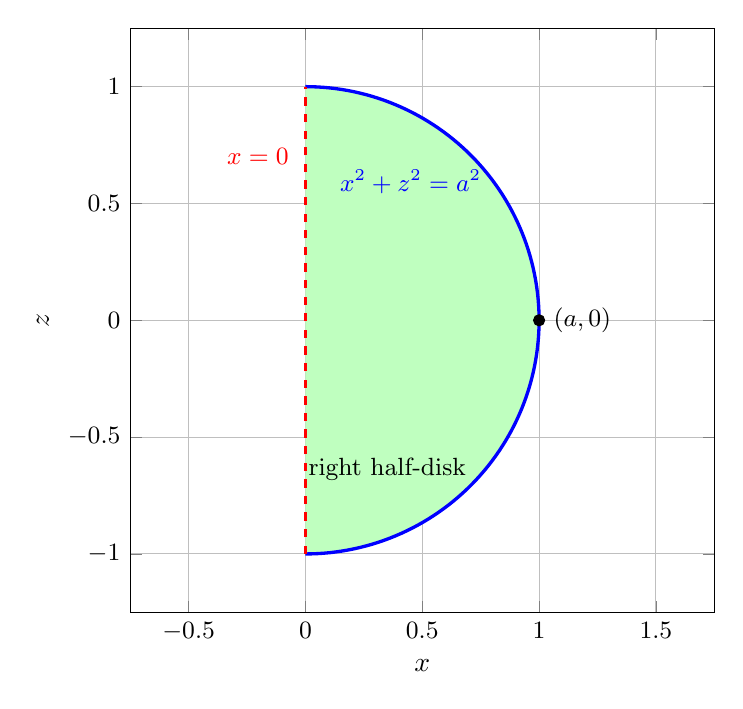
\begin{tikzpicture}
\begin{axis}[
    axis equal,
    xmin=-0.35, xmax=1.35,
    ymin=-1.25, ymax=1.25,
    xlabel=$x$, ylabel=$z$,
    width=9cm, height=9cm,
    grid=major,
    tick label style={font=\small},
]
% Shade the right half-disk cross-section
\addplot[fill=green!25, draw=none, domain=-90:90, samples=120]
    ({cos(x)}, {sin(x)}) -- cycle;

% Sphere arc x^2+z^2=1, x>=0
\addplot[blue, very thick, domain=-90:90, samples=120]
    ({cos(x)}, {sin(x)});

% Cylinder boundary x=0
\addplot[red, very thick, dashed] coordinates {(0,-1) (0,1)};

% Point (a,0)
\addplot[only marks, mark=*, mark size=2pt, color=black] coordinates {(1,0)};

\node[anchor=west, font=\small] at (axis cs:1.02,0) {$(a,0)$};
\node[anchor=east, font=\small, color=red] at (axis cs:-0.03,0.7) {$x=0$};
\node[anchor=south, font=\small, color=blue] at (axis cs:0.45,0.5) {$x^2+z^2=a^2$};
\node[anchor=north, font=\small] at (axis cs:0.35,-0.55) {right half-disk};
\end{axis}
\end{tikzpicture}
\end{document}
